\section{Streaming}
\subsection{Gstreamer}
\label{sec:gstreamer}
As described in Section~\ref{sec:tools_streaming} the tool Gstreamer is used for reading the drones' video feed and forwarding it to CRTMP.
It is a pipeline based tool, and can be run through the command line using the \verb+gst-launch-0.10+ command.
A pipeline in gstreamer is a set of plugins the video feed is processed by seperated by a \verb+!+.
The first plugin in the pipeline is called a source element, and the final element a sink.
The plugins between the source and sink element consist of a set of video and audio processing plugins, such as decoders and encoders.

\begin{figure}[htb]
    \centering
    
\includegraphics[width=\textwidth]{gfx/sample_pipeline.pdf}
    \caption{Illustration of a sample pipeline.}
    \label{fig:sample_pipeline}
\end{figure}

The source element is capable of receiving a video feed via a specific protocol from a defined destination.
As described in Appendix~\ref{app:ar_drone_specification} the drone outputs its video feed using TCP on port 5555, and its IP on its network is 192.168.1.1.
To read the stream the Gstreamer plugin \verb+tcpclientsrc+ is used.
The parameters \verb+host+ and \verb+port+ can be set for \verb+tcpclientsrc+ and the first part of the pipeline can be seen in Listing~\ref{lst:tcpclientsrc}.

\begin{lstlisting}[style=sourceCode, language=C, caption=tcpclientsrc setup, label=lst:tcpclientsrc]
gst-launch-0.10 tcpclientsrc host=192.168.1.1 port=5555
\end{lstlisting}

The data available for the next plugin is H.264 encoded video frames with PaVE headers.
The PaVE headers cannot be interpreted by Flash, and are therefore parsed by gstreamer using the \textit{paveparse} plugin\citep{paveparse}.
Paveparse removes the PaVE headers and send the remaining H.264 data down the pipeline.
Furthermore it handles the delay that comes from the drone using TCP to stream its video feed, by ignoring lost frames, and always displaying the newest received frames.\fxfatal{weak s�tning}.

As specified in Section\fxfatal{skriv det og ref til section tools} the video output of gstreamer should be in FLV.
Two pipelines containing this functionality can be made.
One is using a H.264 decoder to create raw video data, and then encode it as FLV.
The other is using a FLVmux which uses a workaround to convert the H.264 video data to FLV.\fxfatal{D�rlig og ikke helt korrekt s�tning}
The best option is to use the H.264 decoder, however, as the H.264 data has no headers, due to \textit{paveparse}, the FLV encoder cannot properly encode the video data after it has been decoded.
Therefore an FLVmuxer is used to create FLV output.

With FLV encoded video the sink element can be added to the pipeline.
As the video feed is forwarded to CRTMP, the sink element is \verb+rtmpsink+.
It has one parameter called \verb+location+, which is the url of the RTMP server with an extension specifying the url of the stream on the RTMP server\fxfatal{D�rlig s�tning}.
The \verb+rtmpsink+ can be seen in Listing~\ref{lst:rtmpsink}:

\begin{lstlisting}[style=sourceCode, language=C, caption=rtmpsink setup, label=lst:rtmpsink]
rtmpsink location='rtmp://0.0.0.0/live/myStream'
\end{lstlisting}

The pipeline to forward the drones video feed can be seen in Listing~\ref{lst:pipeline1}.

\begin{lstlisting}[style=sourceCode, language=C, caption=Initial Pipeline, label=lst:pipeline1]
tcpclientsrc host=192.168.1.1 port=5555 ! paveparse ! flvmux name=mux ! rtmpsink location='rtmp://0.0.0.0/live/myStream'
\end{lstlisting}

There is however the chance some plugins process data faster than others, causing data to pile up at certain plugins if it is send through unrestricted.
This can be solved using the plugin \verb+queue+.
\verb+queue+ is a data queue that queues data until e.g. the queue reaches a specified size.\fxfatal{source: http://gstreamer.freedesktop.org/data/doc/gstreamer/head/gstreamer-plugins/html/gstreamer-plugins-queue.html}
The queue element is added between every plugin except \verb+tcpclientsrc+ and \verb+paveparse+, as there is no need to queue between the entry point and the first plugin.
The complete pipeline can be seen in Listing~\ref{lst:pipeline2}: 

\begin{lstlisting}[style=sourceCode, language=C, caption=Complete Pipeline, label=lst:pipeline2]
tcpclientsrc host=192.168.1.1 port=5555 ! paveparse ! queue ! flvmux name=mux ! queue ! rtmpsink location='rtmp://0.0.0.0/live/myStream'
\end{lstlisting}

\subsection{C++ RTMP Server}
\label{sec:CRTMP}
As described in \ref{sec:tools_streaming} C++ RTMP Server is used as the server tool between Gstreamer and the flash application.

CRTMP is found at http://www.rtmpd.com and comes in a source package ready to run.
It can be runned with the linux command \verb+sh+, which is the bourne-shell or a compatible shell.

There are four possibilities:

\begin{itemize}
   \item run\_all.sh
   \item run\_all\_deamon.sh
   \item run\_flvplayback.sh
   \item run\_flvplayback\_deamon.sh
\end{itemize}

If the command \verb+sh run_all.sh+ is run, CRTMP will startup using the config file \verb+all.lua+.

The flvplayback was used, because this is the flash streamer application, and the configuration file \verb+flvplayback.lua+ was configured like seen in listing~\ref{lst:flvplayback}.

\begin{lstlisting}[style=sourceCode, language=C, caption=flvplayback.lua configuration, label=lst:flvplayback]
acceptors =
           {
                   {
                           ip="0.0.0.0",
                           port=1935,
                           protocol="inboundRtmp"
                   }
           },
externalStreams =
            {
                   {
                           uri="rtmp://flash.oit.duke.edu/vod/MP4:test/brunswick.m4v",
                           localStreamName="test",
                           forceTcp=true
                   }
            },
\end{lstlisting}


\verb+Acceptors+ define inbound- and \verb+externalStreams+ outbound connections.
Inbound defines which ports CRTMP will let users connect to and \verb+externalStreams+ is the source of the stream.
The sample \verb+externalSteam+ seen in listing~\ref{listing:flvplayback} has a video file on an external server as input, and gives the outbound stream the name \verb+test+.
This test source was used to test if CRTMP was running correctly.
To view the stream Video Lan Client, VLC, was used as it has the same capabilities as flash when it comes to streaming RTMP.

A connection is established with an URL of the format seen in Listing~\ref{lst:server_address}, where the \verb+server address+ is the address of the CRTMP server, the \verb+application+ is the application where CRTMP lookup e.g. live or media, and the \verb+streamName+ is the name of the stream.

\begin{lstlisting}[style=sourceCode, language=C, caption=CRTMP URL Format, label=lst:server_address]
rtmp://[server address]/[application]/[streamName]
\end{lstlisting}

When a user connects to CRTMP and the \verb+application+ is live CRTMP will try to find a live stream that correspond to the link name.
If no such live streams is found CRTMP will look in the media folder and try to find file streams.
If no file stream is found CRTMP are going to wait for the live stream \verb+streamName+.

C++ RTMP Server also uses RSA keys.
It is possible to make users and add these users to realms. This can be used as an extra layer of security but is not used in \projectname{}.

\section{Output stream}
Following the setup of Gstreamer and CRTMP the next step is reading the output stream and displaying it in a Flash application.
Due to the PaVE headers this is however not possible.

\subsection{Issues with PaVE Headers}
\label{sec:issues_with_pave_headers}
The documentation for the PaVE headers can be found at \citep[page. 59-60]{ardrone_developer_guide}.
As described in section~\ref{sec:gstreamer} Flash applications are unable to interpret the PaVE headers, and as a result unable to display a video stream encoded with them.
Therefore they must be removed or replaced with another header for the stream to be readable.
The implemented solution removes them with the \verb+paveparse+ plugin, described in section~\ref{sec:gstreamer}.
Removing the header leaves raw video data, with no information about how to interpret it.
As a result the Flash application, VLC, and other video players are unable to interpret the video data.
An illustration of the PaVE header problem can be seen in Figure~\ref{fig:videoframe}.

\begin{figure}[htb]
    \centering
    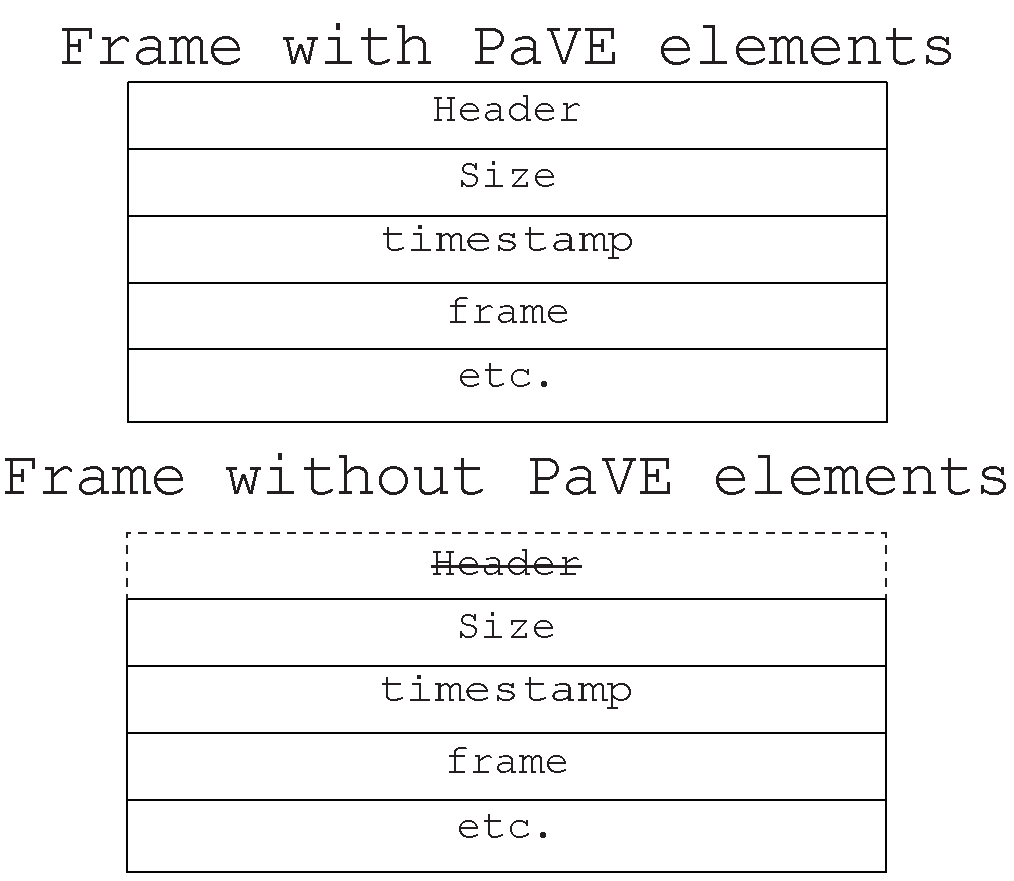
\includegraphics[width=0.7\textwidth]{gfx/videoframe.pdf}
    \caption{Illustration of videoframes with and without PaVe headers.}
    \label{fig:videoframe}
\end{figure}

The PaVE headers result in a situation that makes displaying the video stream in Flash impossible, as the video feed cannot be interpreted by a Flash application both with and without them.

\subsection{Test input}
That the designed solution would work if the drones' video feed used a standard header can be documented by using a different video source.
For this purpose the Gstreamer plugin \verb+videotestsrc+ is used.
It creates a test video stream as seen in figure~\ref{fig:videotestsrc}, consisting of raw video data.


If this source is used instead of the one from the drone it is possible to show that this solution will work.

This solution can be seen in figure~\ref{fig:working_solution}.

\begin{figure}[htb]
    \centering
    
\includegraphics[width=0.6\textwidth]{gfx/testvideosrc.pdf}
    \caption{The test video source played with a Flash application.}
    \label{fig:testvideosrc}
\end{figure}

\begin{figure}[htb]
    \centering
    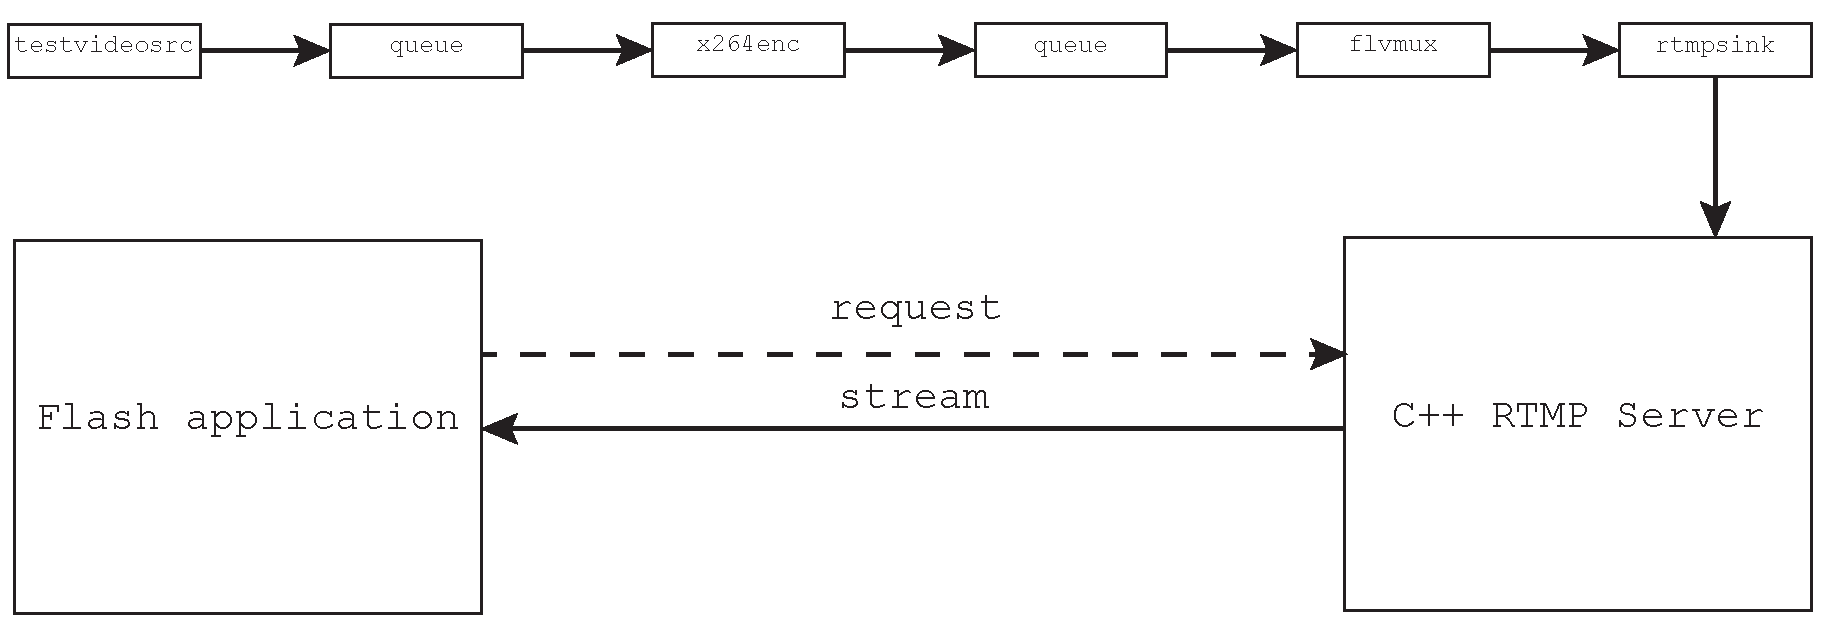
\includegraphics[width=\textwidth]{gfx/Working_solution.pdf}
    \caption{Illustration of the working solution with use of the video test source.}
    \label{fig:working_solution}
\end{figure}

\subsection{Implemented solution}
\label{sec:video_stream_implemented_solution}
The streaming setup used in \projectname{} uses only Gstreamer.
One pipeline which reads the drones' video feed and serves as a server, denoted \deno{SP}, and a client pipeline ,denoted \deno{CP}, for displaying the video feed on the client side.
The setup can be seen in Figure~\ref{fig:current_solution}.

\begin{figure}[htb]
    \centering
    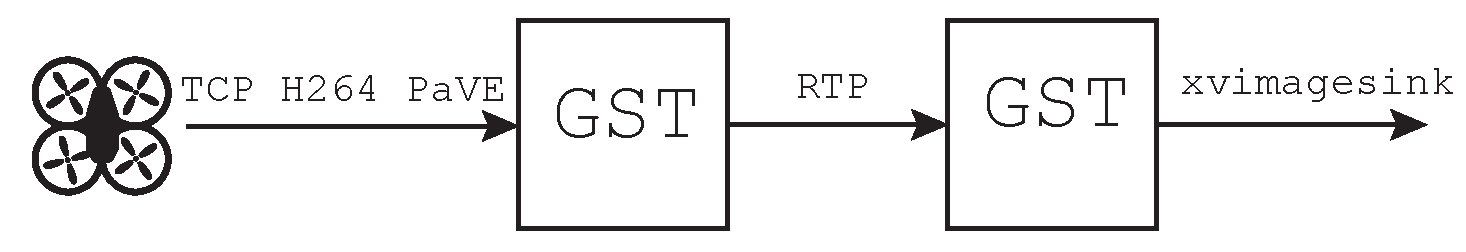
\includegraphics[width=\textwidth]{gfx/current_solution.pdf}
    \caption{Illustration of the current solution with xvimagesink.}
    \label{fig:current_solution}
\end{figure}

\deno{SP} reads the drones' video feed and multicast it using the Real-time Transport Protocol(RTP).
RTP is standardized protocol for sending audio and video packages over IP networks.
RTMP is not used, as it is a protocol made specifically for Flash, and for a Gstreamer only solution RTP is better choice\fxfatal{Hvorfor?}.
RTP packages are sent via UDP.
\deno{SP} uses the \verb+tcpclientsrc+ and \verb+paveparse+ plugins used described in Section~\ref{sec:gstreamer}.

Video data send via RTP must be payloaded, as a video frame is larger than the maximum size allowed size of a UDP packet.
Payloading adds the RTP header to the data packages, which encapsulates the payloaded data.\fxfatal{uspecifikt}
Gstreamer has a set of rtp pay- and depayloaders for each video format it supports.
The plugin used in this pipeline is \verb+rtph264pay+.

Gstreamer does not have a dedicated rtp sink.
As RTP packages are sent via UDP, the \verb+udpsink+ is used.
\verb+udpsink+ has two parameters named \verb+host+ and \verb+port+, and a set of optional flags with default values.
The flag \verb+auto-multicast+ must be set to true to broadcast the stream globally.
Accordingly the host is set to the multicast IP \verb+224.1.1.1+.
The port is set to \verb+5123+ as specified in Section\fxfatal{ref til der hvor det kommer}.

The complete \deno{SP} can be seen in Listing~\ref{lst:SP}:

\begin{lstlisting}[style=sourceCode, language=C, caption=rtmpsink setup, label=lst:SP]
tcpclientsrc host=192.168.1.1 port=5555 ! paveparse ! rtph264pay ! udpsink host=224.1.1.1 port=5123 auto-multicast=true
\end{lstlisting}

\deno{CP} uses the \verb+udpsrc+ element to read the video stream.
\verb+udpsrc+ parameters are identical to those of \verb+udpsink+.
In order to decode the stream, an additional parameter named \verb+caps+ must be set.
\verb+caps+ are used to describe metadata about the incoming video feed, and contains information such as encoding, the protocol it is being sent using, framerate, and more.
The caps are generated by \deno{SP}.
The \verb+udpsrc+ element of \deno{CP} can be seen in Listing~\ref{lst:udpsrc}.

\begin{lstlisting}[style=sourceCode, language=C, caption=udpsrc Setup, label=lst:udpsrc]
udpsrc uri=rtp://XXX.XXX.XXX.XXX port=5123 caps = "application/x-rtp, media=(string)video, clock-rate=(int)90000, encoding-name=(string)H264, sprop-parameter-sets=(string)\"Z01AFeygoP2AiAAAAwALuaygAHixbLA\\=\\,aOvssg\\=\\=\", payload=(int)96, ssrc=(uint)1171155755, clock-base=(uint)868988588, seqnum-base=(uint)65233"
\end{lstlisting}
\fxfatal{Highlighting er m�rkelig i streaming listings}.

The next two steps of the pipeline depayload the received data and decode it to raw video data.
The depayloading is done with the \verb+rtph264depay+ plugin and the decoding with the \verb+ffdec_h264+ plugin.
Following these two steps the video data has reassembled after the transfer and been decoded.
The last plugin used is \verb+xvimagesink+ which displays the video stream to the user.
\verb+xvimagesink+ has two flags used to remove delay on the stream named \verb+sync+ and \verb+async+ which are both set to true.
The complete \deno{CP} can be seen in Listing~\ref{lst:CP}.

\begin{lstlisting}[style=sourceCode, language=C, caption=Client Pipeline, label=lst:CP]
udpsrc uri=rtp://XXX.XXX.XXX.XXX port=5123 caps = "application/x-rtp, media=(string)video, clock-rate=(int)90000, encoding-name=(string)H264, sprop-parameter-sets=(string)\"Z01AFeygoP2AiAAAAwALuaygAHixbLA\\=\\,aOvssg\\=\\=\", payload=(int)96, ssrc=(uint)1171155755, clock-base=(uint)868988588, seqnum-base=(uint)65233" ! rtph264depay ! ffdec_h264 ! xvimagesink sync=false async=false
\end{lstlisting}



%% http://wiki.rtmpd.com/documentation (Maybe this should in bib)